\documentclass{beamer}
\usepackage[T2A]{fontenc}
\usepackage[utf8]{inputenc}
\usepackage[russian]{babel}

\graphicspath{{img/}}
\usepackage{multicol}
\usetheme{JuanLesPins}

\usepackage{amsmath, amsthm, amssymb}
%% листинги кода
\usepackage{listings}
\usepackage{courier}
\lstset{
  language=c++,
  basicstyle=\footnotesize\sffamily,
  keywordstyle=\bfseries,
  stringstyle=\ttfamily,
  numberstyle=\tiny,
  numbers=left
}

\usepackage{moreverb}
\usepackage[noend]{algorithmic}
\algsetup{indent=2em, linenosize=\tiny, linenodelimiter=}

\newcommand{\code}[1]{\textsf{#1}}

% Хак :(
\setbeamertemplate{title page}
{
	\vbox{}
	\vskip1em\par
	\begin{centering}
		\begin{beamercolorbox}[sep=8pt,center,default,rounded=true,shadow=true]{institute}
			\usebeamerfont{institute}\insertinstitute
		\end{beamercolorbox}
		\vfill
		\vfill
		\vfill
		\begin{beamercolorbox}[sep=8pt,center,default,rounded=true,shadow=true]{title}
			\usebeamerfont{title}\inserttitle\par%
			\ifx\insertsubtitle\@empty%
			\else%
				\vskip0.25em%
				{\usebeamerfont{subtitle}\usebeamercolor[fg]{subtitle}\insertsubtitle\par}%
			\fi%     
		\end{beamercolorbox}%
	\end{centering}
	\vskip1em\par
	\begin{beamercolorbox}[sep=8pt,center,default,rounded=true,shadow=true]{author}
		\begin{flushright}
			\tiny{\usebeamerfont{author}\insertauthor}
		\end{flushright}
	\end{beamercolorbox}
	\begin{centering}	
	\end{centering}
	\vfill
}

\title{Восстановление определений классов на языке Си++ посредством динамического анализа бинарного кода}
\author[Пётр Прохоренков]{Прохоренков~П.В.\\гр. 527\vskip0.7cmНаучный~руководитель\\к.ф-м.н,~доц.~Чернов~А.В.}
\institute{Факультет ВМиК\\Кафедра системного программирования}
\date{}

\begin{document}

\begin{frame}[plain]
\titlepage
\end{frame}

\section{Введение}
\begin{frame}
\frametitle{Введение}
\begin{Large}
\begin{enumerate}
	\item \alert{Декомпиляция} --- получение по программе на языке ассемблера эквивалентной программы на языке высокого уровня.
	\item \alert{Восстановление составных типов данных} --- подзадача декомпиляции.
    \item \alert{Восстановление полиморфных иерархий} --- подзадача восстановления типов.
\end{enumerate}
\end{Large}
\end{frame}

\section{Постановка задачи}
\begin{frame}
\frametitle{Постановка задачи}
\begin{Large}
Инструментальное средство должно восстанавливать:
\begin{enumerate}
\item Множество классов.
\item Частичное отношение наследования между классами.
\item Таблицы виртуальных функций для каждого из классов.
\end{enumerate}
\end{Large}
\end{frame}

\section{Метод решения}
\begin{frame}
\frametitle{Обзор}
\begin{Large}
\begin{itemize}
    \item Если есть RTTI, задача сводится к разбору этих структур.
    \item Часто RTTI отсутствует.
    \item Исследуем места вызовов виртуальных функций.
    \item Собираем информацию о <<взаимозаменяемости>> классов.
\end{itemize}
\end{Large}
\end{frame}

\begin{frame}
\frametitle{Средство для анализа кода}
\begin{Large}
\alert{Valgrind} --- среда для динамической бинарной инструментации.
\begin{enumerate}
    \item Исполняемый код $\longrightarrow$
    \item Декомпилированный во внутреннее представление код $\longrightarrow$
    \item Инструментация кода $\longrightarrow$
    \item Компиляция инструментированного кода и выполнение.
\end{enumerate}
\end{Large}
\end{frame}

\subsection{Сбор информации}

\begin{frame}[fragile]
\frametitle{Сбор информации}
Выявление вызовов виртуальных функций с помощью сопоставления с образцом.
\begin{columns}
	\begin{column}[T]{0.45\textwidth}
        \begin{lstlisting}[language={[x86masm]Assembler}]
mov    -0x28(%rbp),%rax
mov    (%rax),%rax
mov    (%rax),%rdx
mov    -0x28(%rbp),%rax
mov    %rax,%rdi
callq  *%rdx
        \end{lstlisting}
    \end{column}
    \begin{column}[T]{0.45\textwidth}
        \center{Пример вызова виртуальной функции на платформе \code{x86\_64}}
    \end{column}
\end{columns}
Если сопоставление успешно, получаем тройку: адрес объекта, указатель на таблицу виртуальных функций, смещение виртуальной функции в таблице
\end{frame}


\begin{frame}[fragile]
\frametitle{Нахождение начала таблицы виртуальных функций}
\begin{columns}
\begin{column}[T]{0.45\textwidth}
\begin{lstlisting}
class A {
public:
    int a;
    virtual void v();
};

class B {
public:
    int b;
    virtual void w();
};

class C : public A, public B {
public:
    int c;
    void w();
};
\end{lstlisting}
\end{column}
\begin{column}[T]{0.45\textwidth}
\begin{figure}
  \center
  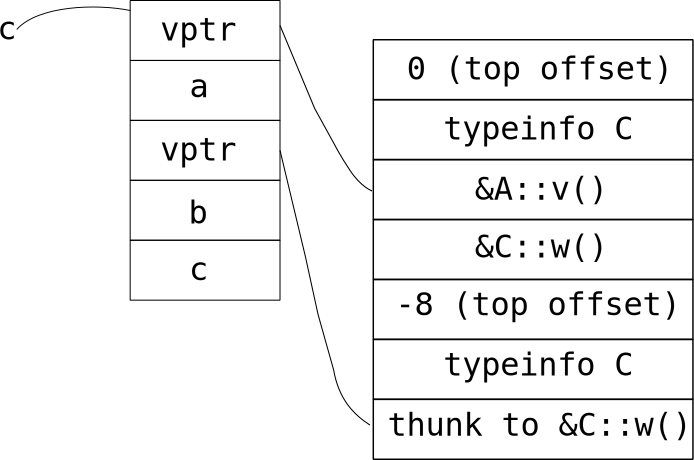
\includegraphics[width=5cm]{multiple_inheritance_scheme.pdf}
  \hfill
\end{figure}
\end{column}
\end{columns}
\end{frame}

\subsection{Построение иерархии}
\begin{frame}
\frametitle{План}
\begin{itemize}
    \item Существует отображение: место виртуального вызова $\rightarrow$ тип данных.
    \item Множество таблиц виртуальных функций, использованных в точке вызова будем обозначать $calles[A]$, номер вызываемой функции $fn[A]$, отношение наследования $A \to B $, неявное наследование $ A \rightsquigarrow B$.
    \item Будем постепенно отождествлять некоторые места вызовов и проставлять отношения наследования.
    \item Условия:
    \begin{itemize}
    \item Тип может иметь только один базовый тип. Множественное наследование выявляется позже, используя информацию о вхождении таблиц виртуальных функций друг в друга.
    \item Считаем, что в типе (классе), соответствующему месту вызова $A$ определено ровно $fn[A]$ виртуальных функций.
    \end{itemize}
\end{itemize}
\end{frame}

\subsubsection{Алгоритм}

\begin{frame}
\frametitle{Продвижение множеств использованных таблиц виртуальных функций}
\begin{eqnarray*}
\forall A,\;B:\qquad callees[A] \cap callees[B] \neq \varnothing \wedge fn[A] \geq fn[B]\\
\implies callees[A] := callees[A] \cup callees[B]
\end{eqnarray*}
\begin{center}
    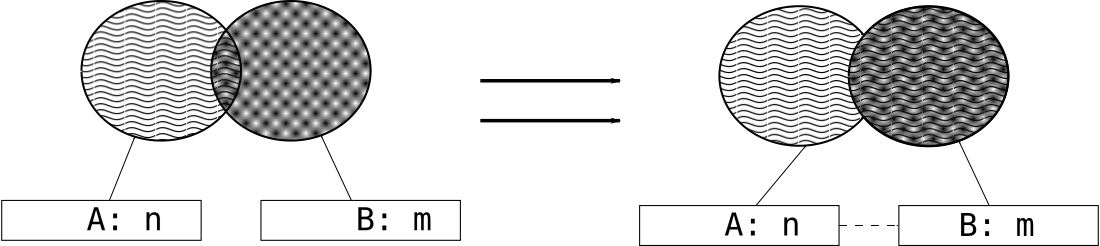
\includegraphics[width=10cm]{callees_propagation.pdf}
\end{center}
\end{frame}

\begin{frame}
\frametitle{Слияние мест вызовов}
\begin{eqnarray*}
\forall A,\;B\qquad fn[A] = fn[B] \wedge callees[A] \cap callees[B] \neq \varnothing\\
\implies A := B
\end{eqnarray*}
\begin{center}
    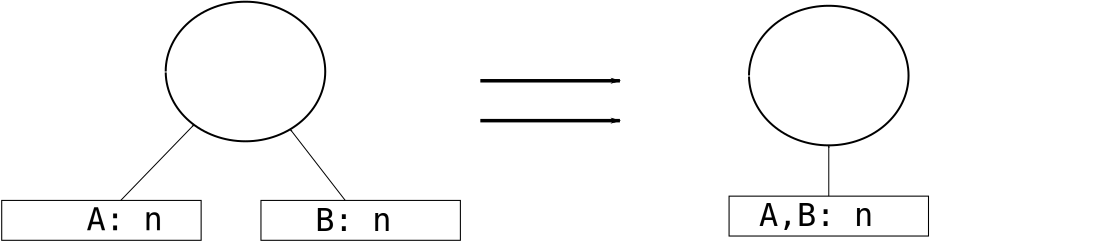
\includegraphics[width=10cm]{call_site_merging.pdf}
\end{center}
\end{frame}

\begin{frame}
\frametitle{Сортировка мест вызовов}
\begin{columns}
\begin{column}[T]{0.45\textwidth}
\begin{eqnarray*}
\forall A\qquad A \rightarrow \begin{cases}
\varnothing,\; \overline{\exists} B:\; A \rightsquigarrow B,\\
\arg\min\limits_{B:\; A \rightsquigarrow B}fn[B]
\end{cases}
\end{eqnarray*}
\end{column}
\begin{column}[T]{0.45\textwidth}
\begin{center}
    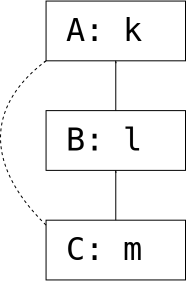
\includegraphics[width=3cm]{call_site_sort.pdf}
\end{center}
\end{column}
\end{columns}
\end{frame}

\begin{frame}
\frametitle{Сокращение цепочек}
\begin{eqnarray*}
\forall A,\;B:\qquad A \rightarrow B\;\wedge\;|\{C:\; C \rightarrow B\}| = 1\\
\implies B := A
\end{eqnarray*}
\begin{center}
    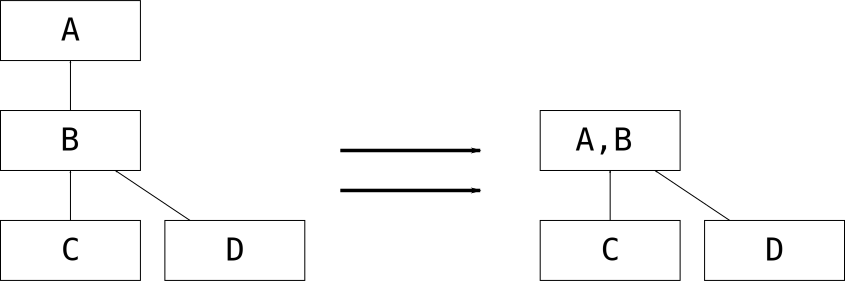
\includegraphics[width=10cm]{chain_fold.pdf}
\end{center}
\end{frame}

\section{Заключение}

\begin{frame}
\frametitle{Пример работы}
Браузер \code{rekonq}. Замедление работы примерно в $2$--$3$ раза.
\vspace{0.5cm}
\begin{center}
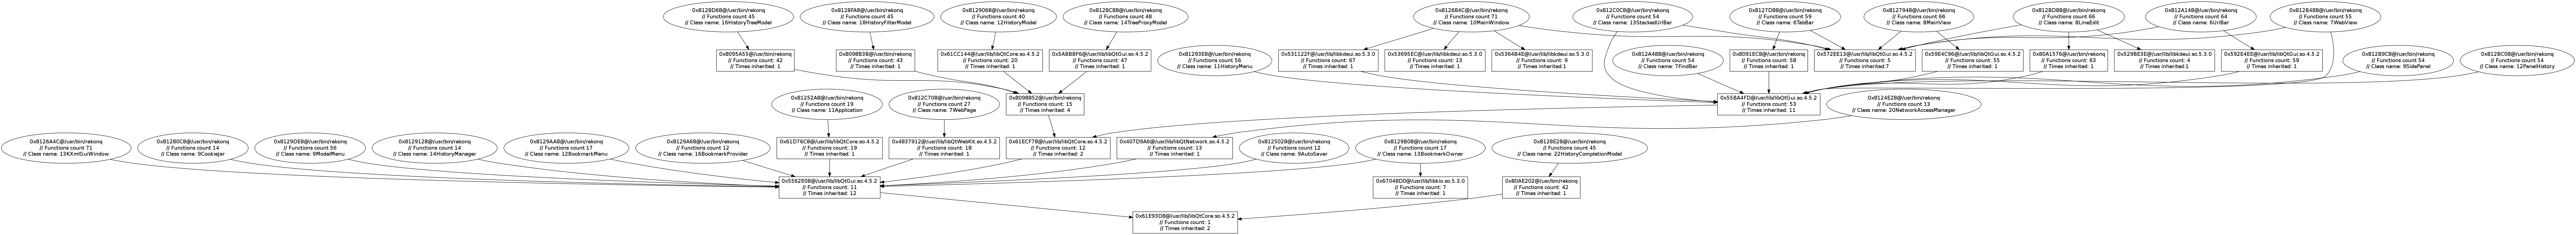
\includegraphics[width=10cm]{rekonq-hier.png}
\end{center}
\vspace{0.5cm}
\begin{center}
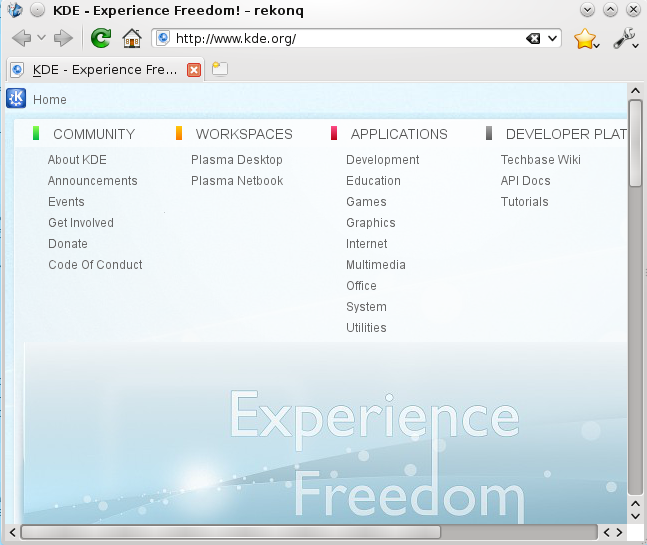
\includegraphics[width=5cm]{rekonq.png}
\end{center}
\end{frame}

\begin{frame}
\frametitle{Заключение}
\begin{Large}
\begin{itemize}
\item Показана возможность применения динамического анализа для восстановления полиморфных типов данных.
\item Разработаны и реализованы методы:
\begin{itemize}
    \item Выявление динамических вызовов во время работы программы.
    \item Построения возможной иерархии классов.
\end{itemize}
\end{itemize}
\end{Large}
\end{frame}

\end{document}
